\section{Introduction to Android}

\begin{breakbox}
\boxtitle{Android Thinking - Design}

In Android application pertain to \textbf{loosely bound components} and
they can easily be \textbf{reused}. The \textbf{system manages these
applications} (register privileges, lifecycle, etc.)

\textbf{Components can be built on its own, or can be used from other
applications}

\end{breakbox}

\begin{breakbox}
\boxtitle{Intents}

Android employs so called \textbf{Intents} to notify components or to
transfer control. An intent itself is a \textbf{passive data structure} holding
an abstract description of an operation to be performed (e.g.~VIEW
something). The system matches an Intent with the component that is most
suitable.
\end{breakbox}

\begin{breakbox}
\boxtitle{AndroidManifest.xml}

This File describes the properties of an application: 
\begin{itemize}
    \item Name / ID (package)
    \item Version of the application
    \item Technical user (sharedUserId) 
    \item Required SDK version 
    \item Required privileges
    \item White list of ``uses''
    \item permissions
    \item Components
    \item Description including list of the Intents the components can receive
\end{itemize}

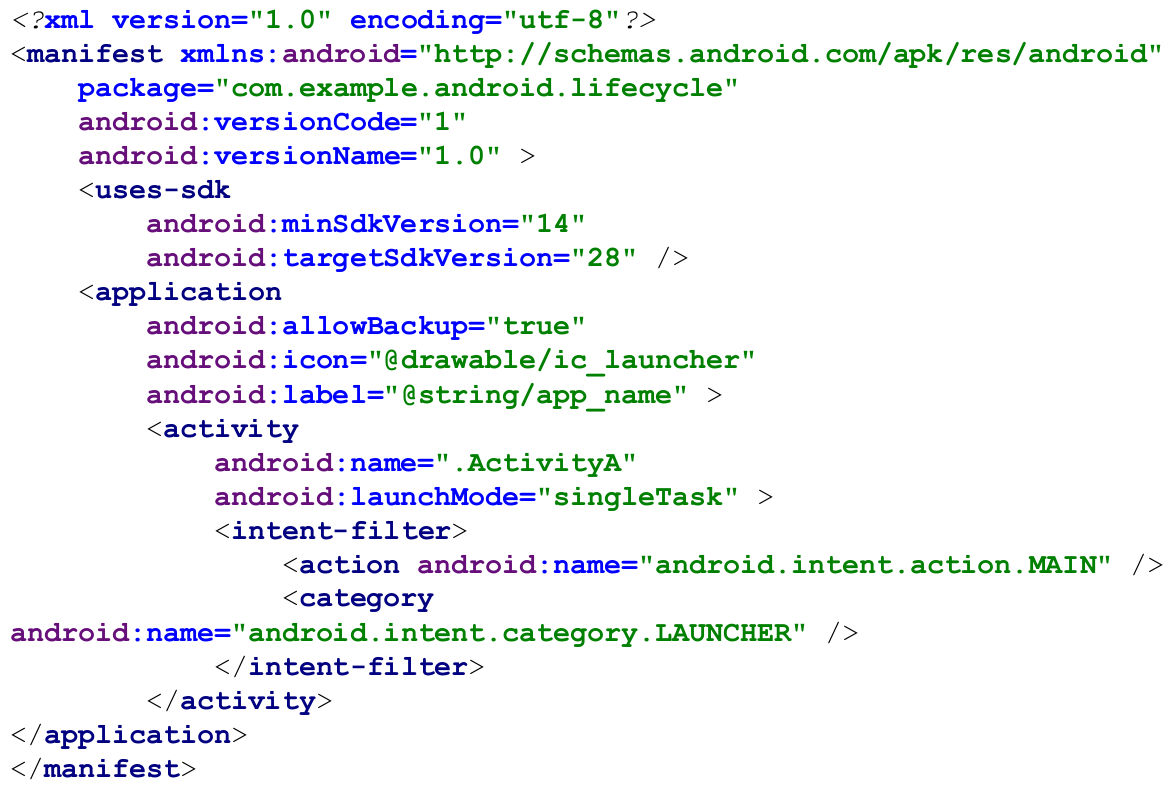
\includegraphics[width=0.24\textwidth]{figures/androidManifest.png}

\end{breakbox}

\subsection{Android Architecture}
\begin{breakbox}
\boxtitle{Android Architecture Overview}

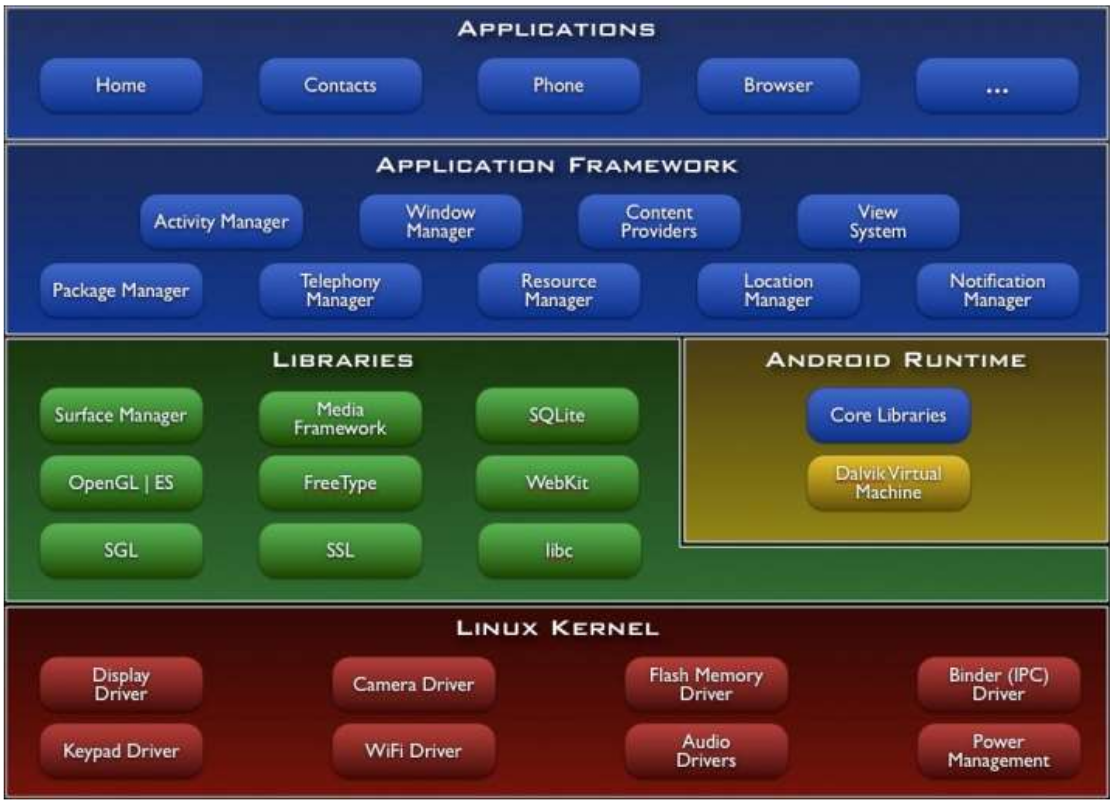
\includegraphics[width=0.24\textwidth]{figures/architectureOverview.png}

\end{breakbox}

\begin{breakbox}
\boxtitle{Linux Kernel}

The Linux Kernel works as a \textbf{hardware abstraction layer (HAL)}.
It has 

\begin{itemize}
    \item device drivers
    \item memory management
    \item process management
    \item networking
\end{itemize}

\end{breakbox}

\begin{breakbox}
\boxtitle{Libraries}

\begin{itemize}
\tightlist
\item
  C/C++ libraries
\item
  Interface through Java
\item
  Surface manager (UI Handling)
\item
  2D and 3D graphics
\item
  Media codecs, SQLite, Browser engine
\end{itemize}

\end{breakbox}

\begin{breakbox}
\boxtitle{Android Runtime}

\begin{itemize}
\tightlist
\item
  Executes the executables translated from Java bytecode
\item
  Garbage collections, debugging
\item
  Optimized
\item
  Core Libraries
\end{itemize}

\end{breakbox}

\begin{breakbox}
\boxtitle{Application Framework}

\begin{itemize}
\tightlist
\item
  API
\item
  Activity Manager
\end{itemize}

\end{breakbox}

\subsection{Application Building Blocks}

\begin{breakbox}
\boxtitle{Activity}

User interface component typically corresponding to one screen. An
application typically consists of several screens. Activities are
implemented by extending the Activity class.

\end{breakbox}

\begin{breakbox}
\boxtitle{Service}

A service does not have a visual user interface, but rather runs in the
background for an indefinite period of time (e.g.~music player, network
download, etc.).

\end{breakbox}

\begin{breakbox}
\boxtitle{Broadcast Receiver}

Component that receives and reacts to broadcast announcements. E.g.,
announcements that the time zone has changed, that the battery is low.
Broadcast receivers are implemented extending the BroadcastReceiver
class. \textit{(Broadcast announcements are Intents, too.)}

\end{breakbox}

\begin{breakbox}
\boxtitle{Content Providers}

Using a content provider is the \textbf{recommended way to share data
between Android applications}. Any content is represented by URI and
MIME type. Applications do not call content providers directly. They
call ContentResolvers instead as they typically do not reside in the
same process.

\end{breakbox}

\subsection{Transferring Control among Activities}

\begin{breakbox}
\boxtitle{Code Example}
\begin{lstlisting}
public void onClickSendBtn(final View btn){
    Intent intent = new Intent(this, Receiver.class);
    intent.putExtra("msg", "Hello World");
    startActivity(intent);
}
//Sub-activity being called
public void onCreate(Bundle savedInstanceState){
    ...
    Intent intent = getIntent();
    String msg = intent.getExtras(). getString("msg");
    displayMessage(msg);
}
\end{lstlisting}
\end{breakbox}

\begin{breakbox}
\boxtitle{Explanation}
\begin{itemize}
\tightlist
\item
  Android uses a requestId to differentiate among multiple invocations
  of a sub-activity and an intent to return data
\item
  Calling the sub-activity\\
  startActivityForResult(intent, requestId) or\\
  startActivity(intent)
\item
  Returning a result from the sub-activity\\
  etResult(resultCode, intent)\\
  finish()
\item
  Processing the result\\
  onActivityResult(requestId, resultCode, intent)
\item
  Calling Activity\\
  startActivityForResult(new Intent(this, ActivityA.class), id1);\\
  startActivityForResult(new Intent(this, ActivityB.class), id2);
\item
  Processing the result
\end{itemize}
\end{breakbox}

\begin{breakbox}
\boxtitle{Result Handling}
\begin{lstlisting}
@Override
protected void onActivityResult(int requestCode, int resultCode, Intent data) {
    switch (requestCode) {
        case id1: // Process result from invocation with id1
            if (resultCode == RESULT_OK) { /* process data */ }
            break;
        case id2: // Process result from invocation with id2
            if (resultCode == RESULT_OK) { /* process data */ }
            break;
    }
}
\end{lstlisting}
\end{breakbox}


\subsection{Activity Lifecycle}
\begin{breakbox}

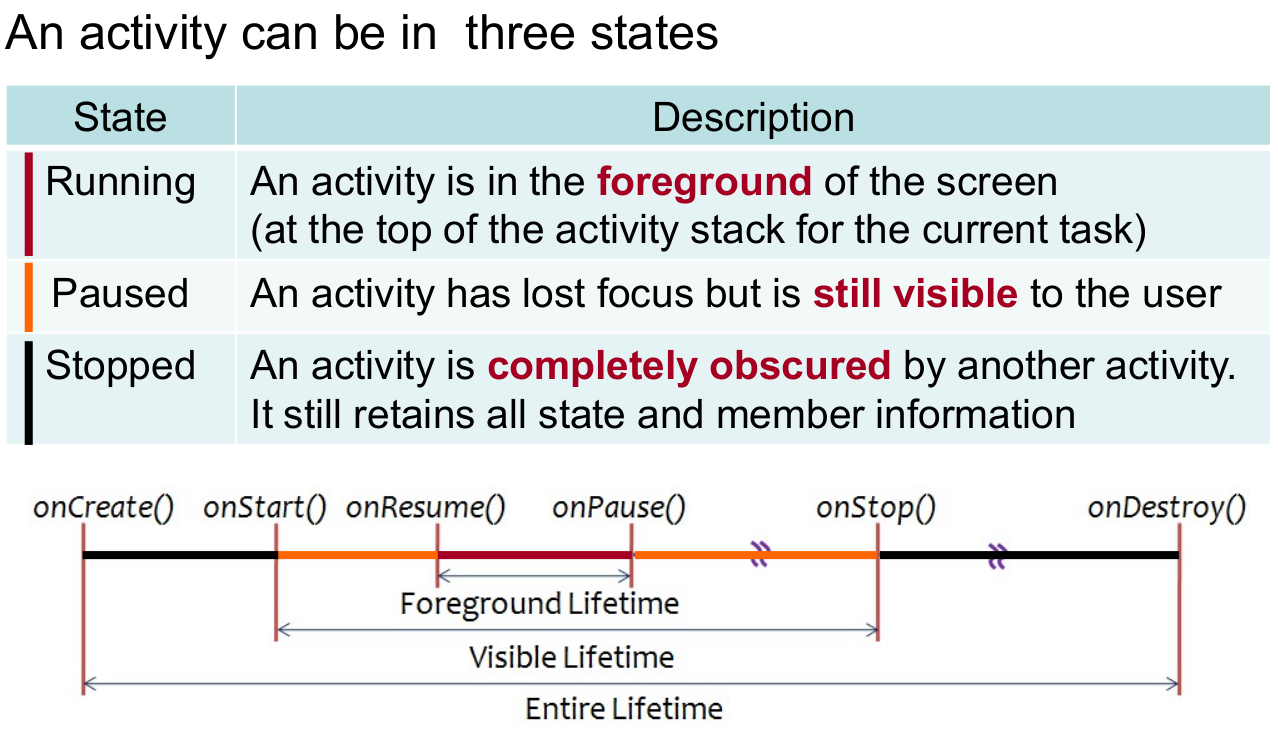
\includegraphics[width=.24\textwidth]{figures/activityLifecycle.png}
\end{breakbox}

\subsection{Resources}
\begin{breakbox}

To optimize access, \textbf{resources (should be done in xml) are
compiled} into the final android package (APK) file and stored in object
trees. These objects can be acessed from Java code.

\textbf{During application development} resources are stored in the res
directory of your project and \textbf{are grouped} according to type:
drawable, layout, values.
\textbf{At build time} the Android resource compiler, i.e., the Android
Asset Packaging Tool aapt, generates a \textbf{wrapper class called R}
that contains resource IDs (static integer) that can be employed to
access the resources in Java with the syntax:\\
\emph{R.resource\_type.resource\_name}
\end{breakbox}
